\documentclass[12pt,letterpaper]{article}

\usepackage{times}
\usepackage{amsmath,amsfonts}
\usepackage{graphicx}
\usepackage{setspace}
\usepackage{indentfirst}
\usepackage{url}

% revise margins
\setlength{\headheight}{0.0in}
\setlength{\headsep}{0.0in}
\setlength{\topmargin}{0.0in}
\setlength{\textheight}{8.9in}
\setlength{\footskip}{0.4in}
\setlength{\oddsidemargin}{0.0in}
\setlength{\evensidemargin}{0.0in}
\setlength{\textwidth}{6.5in}

\setlength{\rightskip}{0pt plus 1fil} % makes ragged right


% for the link to the data at QTL Archive
\usepackage{hyperref}
\hypersetup{pdfpagemode=UseNone} % don't show bookmarks on initial view
\hypersetup{hidelinks}


%bibliography format
\usepackage[authoryear]{natbib}
\bibpunct{(}{)}{;}{a}{}{,}

% hanging environment for Figure legends
\newenvironment{hanging}
{\begin{list}{}
        {\setlength{\labelwidth}{0in}
         \setlength{\leftmargin}{1em}
         \setlength{\itemindent}{-1em}
        }
}
{\end{list}}

%\usepackage{Sweave}
\begin{document}
\setstretch{2.0}

\vspace*{8mm}
\begin{center}

\textbf{\Large R/qtlcharts: interactive graphics \\
  for quantitative trait locus mapping}

\bigskip \bigskip \bigskip \bigskip

{\large Karl W. Broman$^1$}

\bigskip \bigskip

Departments of Biostatistics and Medical Informatics,
\\ University of Wisconsin--Madison, Madison, Wisconsin 53706
\end{center}


\vfill

\hfill
{\footnotesize 13 Nov 2014}

\newpage

\noindent \textbf{Running head:} Interactive QTL graphics


\bigskip \bigskip \bigskip

\noindent \textbf{Key words:} QTL, data visualization, software, D3


\bigskip \bigskip \bigskip

\noindent \textbf{$^1$Corresponding author:}

\begin{tabular}{lll}
 \\
 \hspace{1cm} & \multicolumn{2}{l}{Karl W Broman} \\
 & \multicolumn{2}{l}{Department of Biostatistics and Medical Informatics} \\
 & \multicolumn{2}{l}{University of Wisconsin--Madison} \\
 & \multicolumn{2}{l}{2126 Genetics-Biotechnology Center} \\
 & \multicolumn{2}{l}{425 Henry Mall} \\
 & \multicolumn{2}{l}{Madison, WI 53706} \\
 \\
 & Phone: & 608--262--4633 \\
 & Email: & \verb|kbroman@biostat.wisc.edu|
\end{tabular}

\newpage

\centerline{\sffamily \textbf{Abstract}}

Every data visualization can be improved with some level of
interactivity. Interactive graphics hold particular promise for the
exploration of high-dimensional data.  R/qtlcharts is an R
package to create interactive graphics for experiments to map
quantitative trait loci (QTL; genetic loci that influence
quantitative traits). R/qtlcharts serves as a companion to the R/qtl
package, providing interactive versions of R/qtl's static graphs, as
well as additional interactive graphs for the exploration of
high-dimensional genotype and phenotype data.

\newpage

Interactive graphics have enormous value for the exploration of
high-dimensional genetic data. Visualizations of high-dimensional data
must be a compressed summary, but with interactive visualizations,
features may be linked to underlying details or to different views of
the data. Moreover, interactive graphs offer
the ability to zoom into dense figures, and sets
of linked graphic panels offer greater opportunity to make
connections across diverse data types.

Interactive data visualization has a long history. For example, an
early innovation, brushed scatterplots, is due to \citet{Becker1987}.
While numerous tools for interactive data visualization have been
developed, for example Mondrian
\citep[\href{http://www.theusrus.de/Mondrian}{\tt \small http://www.theusrus.de/Mondrian}]{Theus2008}
and SpotFire (\href{http://spotfire.tibco.com/}{\tt \small http://spotfire.tibco.com/}),
until recently interactive visualization has been a specialized craft,
and the tools have not been widely adopted as part of routine data
analysis. But there has been a recent expansion in the general use and
development of complex and rich interactive graphics tools, motivated
in part by the JavaScript library D3
\citep[\href{http://d3js.org}{\tt \small http://d3js.org}]{Bostock2011},
the development of HTML5 and scalable vector graphics (SVG), and the
power of modern web browsers. Moreover, as these graphical tools are
deployed as web pages, they are immediately accessible to users.

R/qtlcharts is add-on package for the general statistical software R
\citep{R} that provides interactive data visualizations for
quantitative trait locus (QTL) mapping experiments. R/qtlcharts is a
companion to R/qtl \citep{Broman2003}, providing interactive versions
of R/qtl's basic static graphics and additional interactive
visualizations for high-dimensional genotype and phenotype data.

For example, Figure~\ref{fig:chart} contains a static view of an
interactive visualization of the results of QTL analysis with a
phenotype measured over time. The data are from
\citet{Moore2013}. Figure~\ref{fig:chart}A contains a heat map of the
LOD scores from a single-QTL genome scan, considering each time point
individually. Hovering over the heat map drives the contents of the
other two panels and also reveals the LOD score values through a
tool-tip. Figure~\ref{fig:chart}B displays the LOD curves across
the genome for the selected time point. Figure~\ref{fig:chart}C
displays the estimated effect, across time, of the putative QTL at the
selected position.

The interactive versions of R/qtl's static graphs provide considerable
value to the user, enabling a deeper and more rapid exploration of
QTL mapping results. The LOD curves from a single-QTL genome scan are
linked to a panel displaying the association between genotype and
phenotype at putative QTL. This lowers the barrier to inspection of
QTL effects. One should not rely solely on test statistics like the
LOD score, but with the extra effort required to generate plots of QTL
effects in R/qtl, such effect plots are sometimes skipped. The
interactive graph of genome scan results can also serve as important
tool for teaching: the easy connection between LOD scores and
estimated QTL effects can help students to develop a better
understanding of QTL analysis results.

A static heat map with the results of a two-dimensional, two-QTL
genome scan can be difficult to interpret.  In the interactive
version, hovering over the heat map with a mouse reveals the
corresponding positions and LOD scores, and mouse click generates
plots of the genotype-phenotype relationship for the pair of putative
QTL, as well as plots of cross-sectional slices through the
two-dimensional image. This interactivity eases the
identification of both interesting QTL effects as well as artifacts (such
as apparent epistatic interactions that are driven by a few
individuals with outlying phenotype values).

One final example: in a static graph of a genetic marker map, the
marker names are often omitted, as they otherwise clutter the
figure. In the interactive version produced by R/qtlcharts, the marker
names and locations are revealed when hovering over the positions, and
there is also a search box for identifying the position of a
specified marker.

The core of R/qtlcharts is a set of modular, reusable graphic panels,
based on the D3 JavaScript library.  Examples of these panels are
displayed in Figure~\ref{fig:panels} and include heat maps, LOD curve
plots, and scatterplots. Multiple panels are combined into
higher-level interactive charts with links among the panels (as in
Figure~\ref{fig:chart}).

With R/qtlcharts, a single line of R code can generate such an
interactive graph: an HTML file is created and opened in a web
browser. The file can be self-contained and so easily shared with
collaborators.

The interactive charts can also be included within R Markdown
documents (\href{http://rmarkdown.rstudio.com}{\tt \small
http://rmarkdown.rstudio.com}). R Markdown is a variant of
the light-weight markup language, Markdown
(\href{http://daringfireball.net/projects/markdown}{\tt \small
http://daringfireball.net/projects/markdown}), with embedded chunks
of R code. An R Markdown document is converted, via knitr
\citep[\href{http://yihui.name/knitr}{\tt \small
http://yihui.name/knitr}]{Xie2013}, to an HTML file with the R
code chunks replaced by their results (including, for example,
figures). This is an example of literate programming
\citep{Knuth1984}, a key tool for ensuring that research results are
reproducible.

The interactive graphics in R/qtlcharts are written in CoffeeScript
(\href{http://coffeescript.org}{\tt \small http://coffeescript.org}),
which is translated to JavaScript but is a more pleasant language for
programming. Tool tips are implemented with d3-tip
(\href{https://github.com/Caged/d3-tip}{\tt \small
https://github.com/Caged/d3-tip}).

Examples and documentation, including installation instructions, are available at the R/qtlcharts website,
\href{http://kbroman.org/qtlcharts}{\tt \small http://kbroman.org/qtlcharts}.
The code is released under the MIT license and is
available at GitHub,
\href{https://github.com/kbroman/qtlcharts}{\tt \small http://github.com/kbroman/qtlcharts}.


\clearpage
\centerline{\sffamily \textbf{Acknowledgments}}
\'Saunak Sen generously provided comments for improvement of the
manuscript.
This work was supported in part by National Institutes of Health grant
R01GM074244.




\clearpage
\bibliographystyle{genetics}
\renewcommand*{\refname}{\centerline{\sffamily \normalsize \textbf{Literature Cited}}}
\bibliography{rqtlcharts}



\newpage



\centerline{\sffamily \textbf{Figure Legends}}

\begin{hanging}

\item \textbf{Figure 1.}
A static view of an interactive graph for QTL analysis
with a phenotype measured over time, with data from \citet{Moore2013}
concerning root gravitropism in Arabidopsis recombinant inbred lines
(RIL), Ler$\times$Cvi.  \textbf{A}: Heat map of signed LOD
scores for single-QTL analysis at each individual time point. Red
indicates that RIL with the Cvi allele have a larger average
phenotype; blue indicates that RIL with the Ler allele have a larger
average phenotype. Panel A is linked to panels B and C: when hovering
over the heat map, the LOD curves for the corresponding time point are
shown below (\textbf{B}), and the estimated QTL effect, as a function
of time, is shown to the right (\textbf{C}).  For the interactive
version of this figure, see
\href{http://kbroman.org/qtlcharts/example}{\tt \small http://kbroman.org/qtlcharts/example}.

\item \textbf{Figure 2.}
Examples of the basic panels that form the core of
R/qtlcharts. \textbf{A}: heat map, \textbf{B}: LOD curves, \textbf{C}:
scatterplot, and \textbf{D}: a set of confidence intervals.

\end{hanging}



\newpage

\begin{figure}[!ht]
\begin{center}
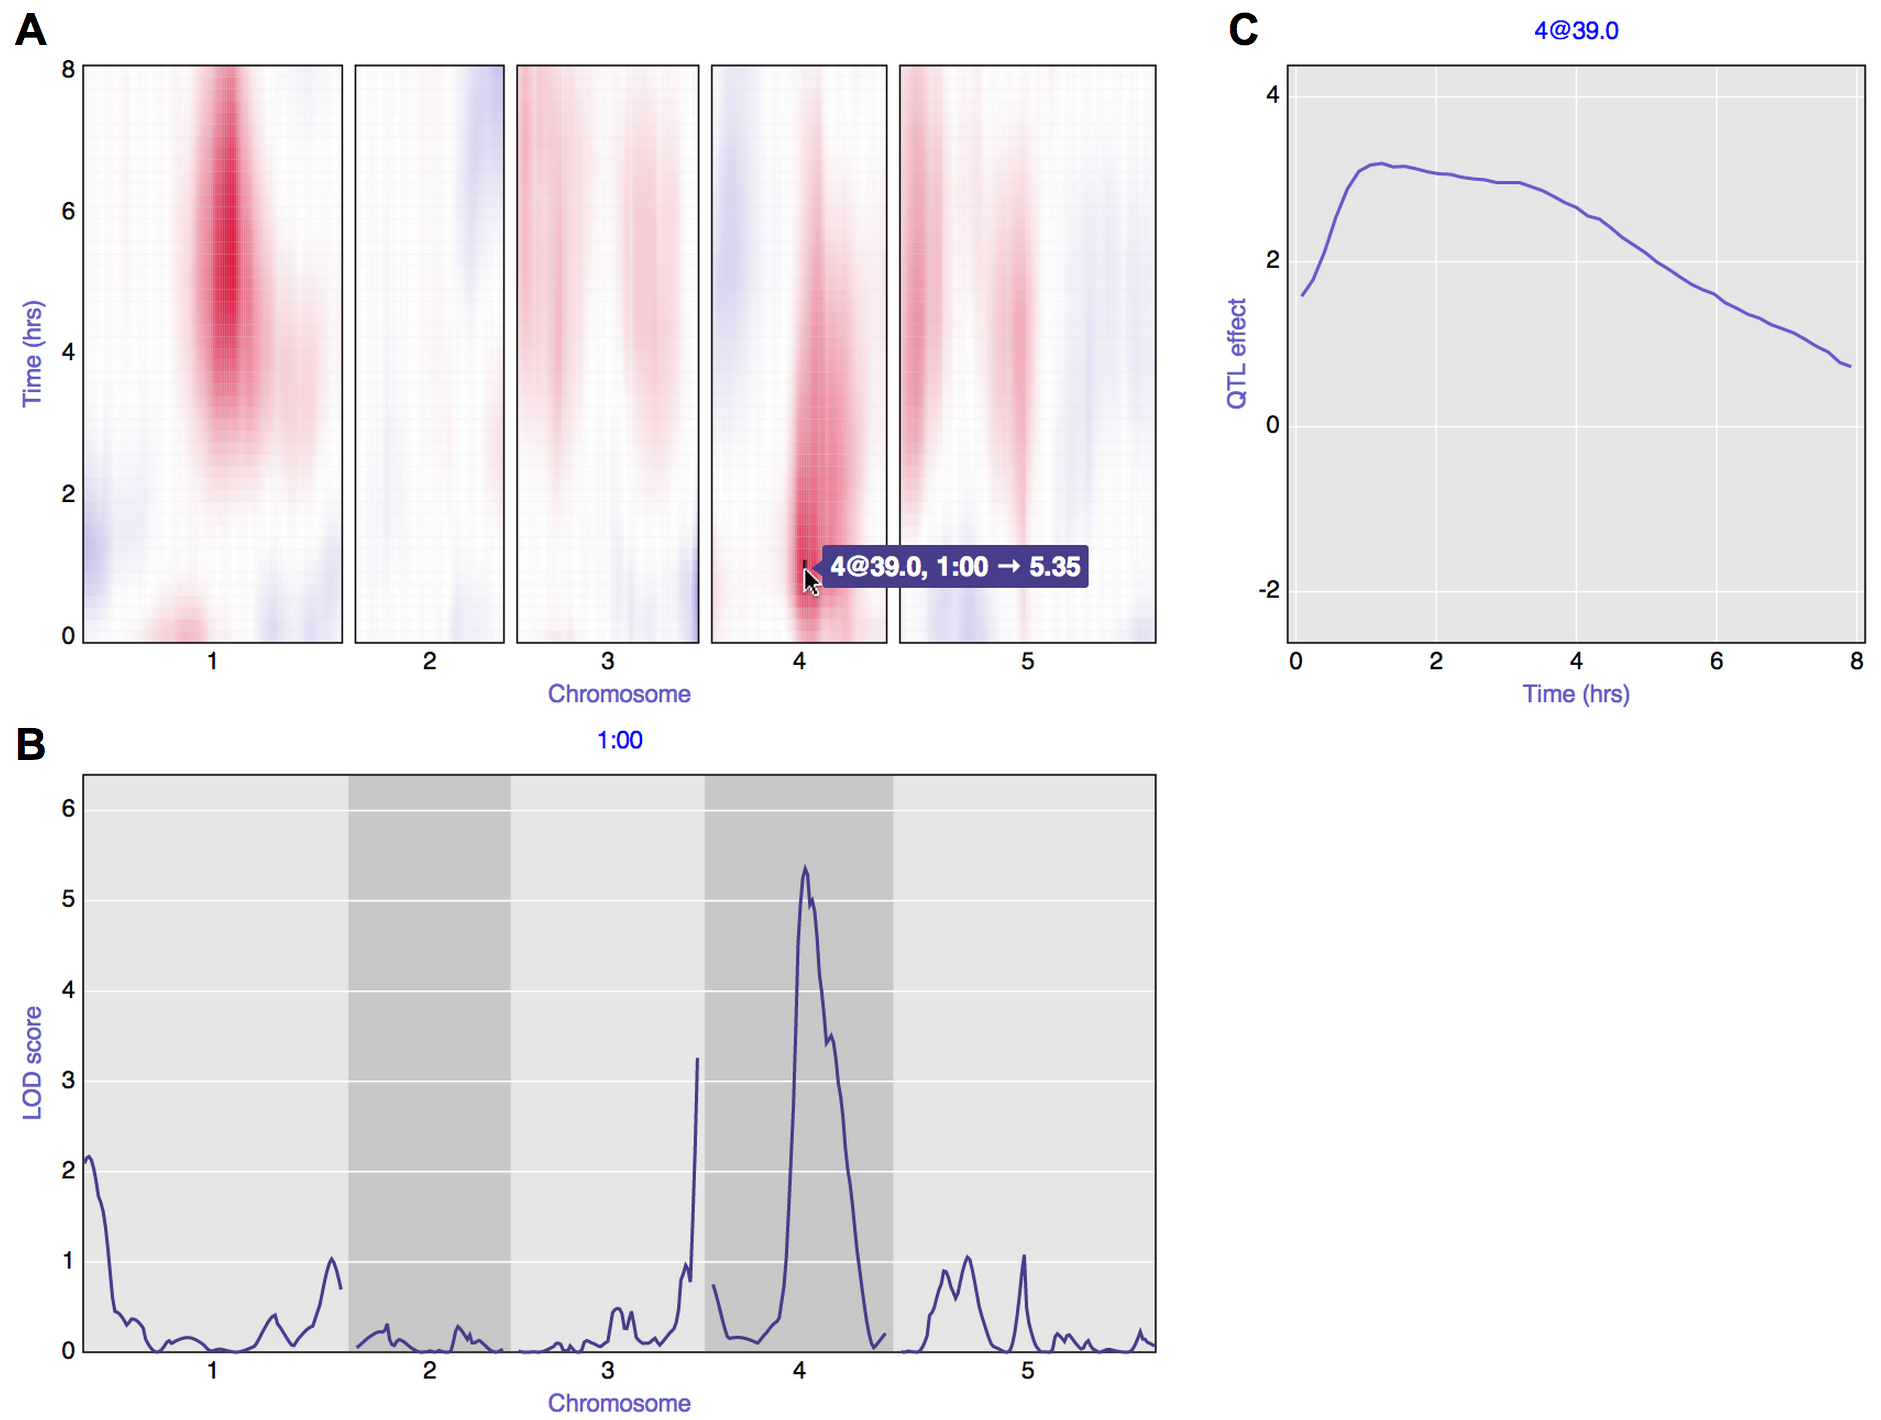
\includegraphics[width=\textwidth]{Figs/fig1.png}
\vspace{1cm}
\caption{
A static view of an interactive graph for QTL analysis
with a phenotype measured over time, with data from \citet{Moore2013}
concerning root gravitropism in Arabidopsis recombinant inbred lines
(RIL), Ler$\times$Cvi.  \textbf{A}: Heat map of signed LOD
scores for single-QTL analysis at each individual time point. Red
indicates that RIL with the Cvi allele have a larger average
phenotype; blue indicates that RIL with the Ler allele have a larger
average phenotype. Panel A is linked to panels B and C: when hovering
over the heat map, the LOD curves for the corresponding time point are
shown below (\textbf{B}), and the estimated QTL effect, as a function
of time, is shown to the right (\textbf{C}).  For the interactive
version of this figure, see
\href{http://kbroman.org/qtlcharts/example}{\tt \small http://kbroman.org/qtlcharts/example}.
\label{fig:chart}
}
\end{center}
\end{figure}


\newpage

\begin{figure}[!ht]
\begin{center}
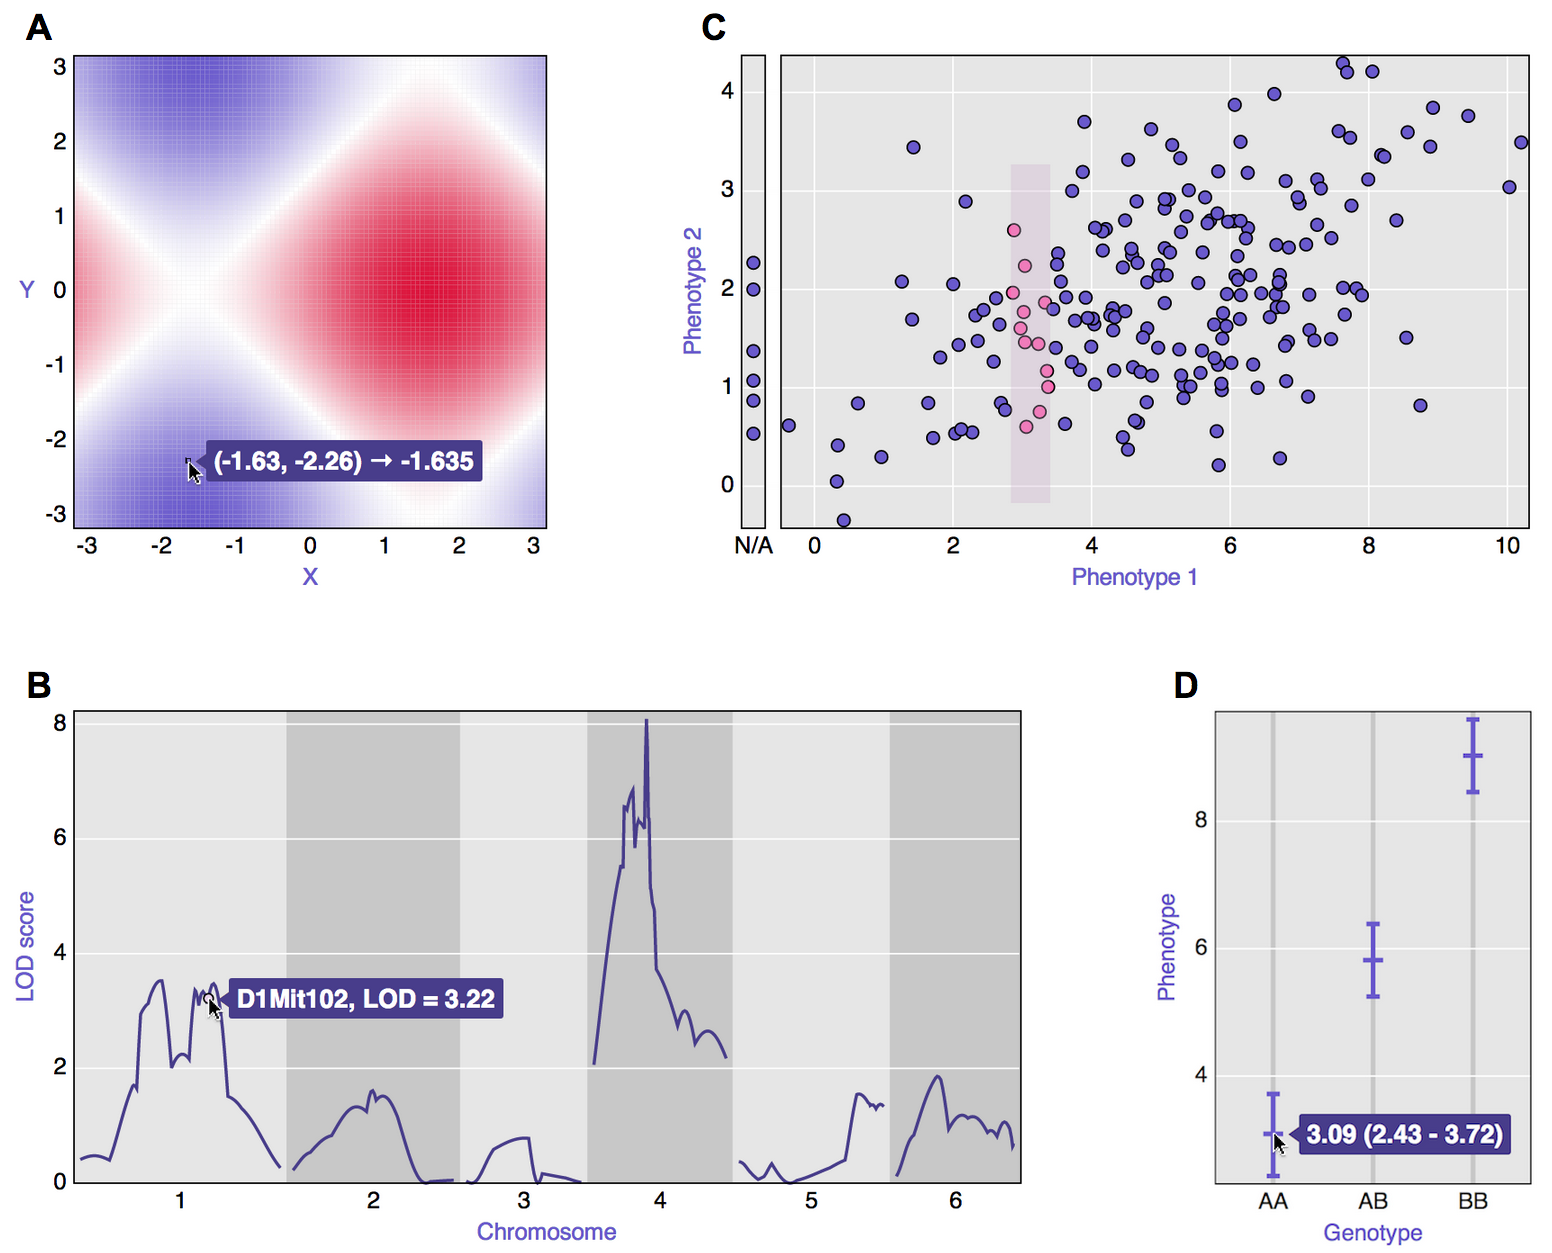
\includegraphics[width=\textwidth]{Figs/fig2.png}
\vspace{1cm}
\caption{
Examples of the basic panels that form the core of
R/qtlcharts. \textbf{A}: heat map, \textbf{B}: LOD curves, \textbf{C}:
scatterplot, and \textbf{D}: a set of confidence intervals.\label{fig:panels}
}
\end{center}
\end{figure}


\end{document}
